\documentclass[a4paper,11.5pt,oneside]{article}

\usepackage{amsmath}
\usepackage{graphicx}

\begin{document}

\title{Treedepth of Control Flow Graphs}
\author{Abolfazl Soltani}
\date{}
\maketitle

\section{Definitions}

Treedepth of a graph $G$ is the minimum height of a tree elimination order of $G$.
It is equivalent to vertex ranking number of $G$ and is denoted by $td(G)$.

\section{Control Flow Graphs}


A basic block is a sequence of instructions with no branches in except to the entry and no branches out except at the exit.
There may be branches within the block, but the branch stays within the block.
One instructions may be in more than one basic block.

A basic block $B_1$ is \textbf{strong} if for any other basic block $B_2$, one of the following conditions holds:
\begin{enumerate}
    \item $B_1 \subseteq B2$
    \item $B_2 \subseteq B1$
    \item $B_1 \cap B_2 = \emptyset$
\end{enumerate}

All strong basic blocks are a laminar family. 
We can construct a tree called \textbf{Strong Basic Blocks Decomposition} (SBBD) from the strong basic blocks 
by adding an edge from $B_1$ to $B_2$ if $B_1 \subset B_2$ and 
there is no $B_3$ such that $B_1 \subset B_3 \subset B_2$. 

\textbf{Claim 1}: For any control flow graph $G$, 
we can construct a tree elimination order with height at most 
$\mathcal{O}(h \log c)$ where $h$ is the height of SBBD and $c$ is maximum number of children of a node in SBBD.

\textbf{Proof}: We construct a tree elimination order of $G$ with induction on the height of SBBD.
For the base case, we consider a tree with height 1 (a node and its children).

$Sub(v)$ is the subtree of SBBD rooted at $v$. $Sub(v)$ is consecutive lines of program.
\textit{Top(v)} is the first line of program in $v$, 
\textit{Bottom(v)} is the last line of program in $v$.
First, we construct a tree elimination order for \textit{Sub(u)} for all children $u$ of $v$.
Then, we construct a tree elimination order for \textit{Sub(v)}. We do this by case analysis on the type of $v$.

\textbf{Case 1}: $Top(v)$ is a branch instruction $if$ and $Bottom(v)$ is the line of the branch instruction.
In this case, we make first and last line of $v$ roots of tree elimination order of $Sub(v)$ and root of $Sub(u_1)$ is child of $fi$ and root of $Sub(u_2)$ is child of $else$. It is shown in figure \ref{fig:case1}.

\begin{figure}[!ht]
\centering
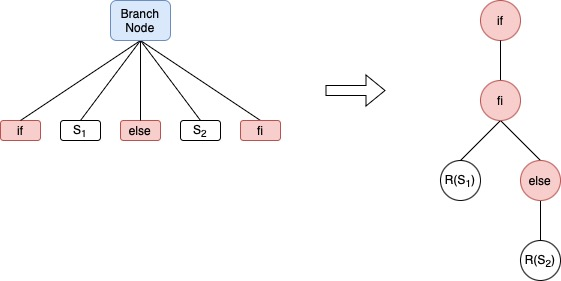
\includegraphics[width=0.5\textwidth]{case1.jpg}
\caption{Case 1}
\label{fig:case1}
\end{figure}

\textbf{Case 2}: $Top(v)$ is a loop instruction $while$ and $Bottom(v)$ is the line of the loop instruction.
In this case, we make first and last line of $v$ roots of tree elimination order of $Sub(v)$ and root of $Sub(u)$ is child of $done$. It is shown in figure \ref{fig:case2}.

\begin{figure}[!ht]
\centering
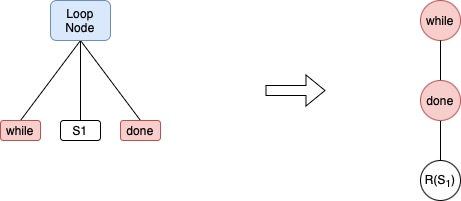
\includegraphics[width=0.5\textwidth]{case2.jpg}
\caption{Case 2}
\label{fig:case2}
\end{figure}

\textbf{Case 3}: In this case, $v$ is a sequence of basic blocks. 
We have to merge tree elimination orders of $Sub(u)$ for all children $u$ of $v$.
Let $u_1, u_2, \dots, u_c$ be children of $v$. First, we merge tree eliminations of $u_1$ and $u_c$, to make sure root and the only child of the root are first and last line of $v$ respectively.
After that, merging tree eliminations of $u_2, u_3, \dots, u_{c-1}$ is similar to tree elimination order of a path. We choose $u_{\frac{c}{2}}$ as root and build tree elimination order of $u_2, u_3, \dots, u_{\frac{c}{2}-1}$ as left subtree and tree elimination order of $u_{\frac{c}{2}+1}, u_{\frac{c}{2}+2}, \dots, u_{c-1}$ as right subtree. It is shown in figure \ref{fig:case3}.

\begin{figure}[!ht]
\centering
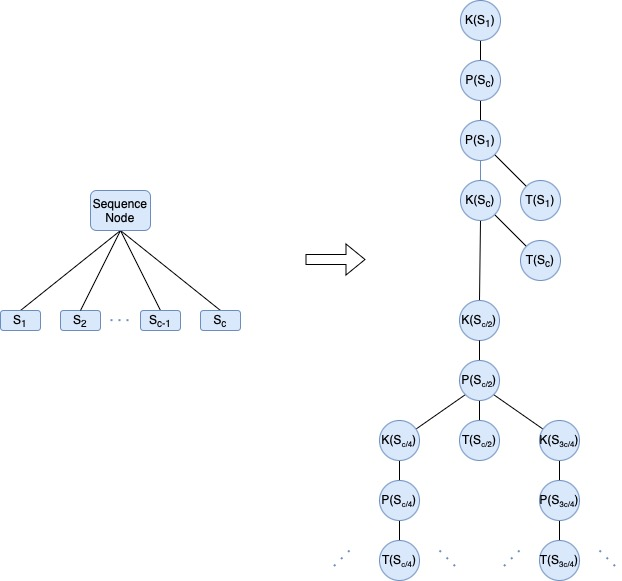
\includegraphics[width=0.5\textwidth]{case3.jpg}
\caption{Case 3}
\label{fig:case3}
\end{figure}

\textbf{Analysis}: Now we proof by induction on the depth of node $v$ that height of tree elimination order of $Sub_v$ is at most $\mathcal{O}(h \log c)$ where $h$ is height of $Sub_v$.
For the base case, we consider a node $v$ with depth 1 that are leaves of SBBD. Now consider a node $v$ with depth $d$. In cases $1$, and $2$, height of tree elimination is at most $\alpha + 3$ where $\alpha$ is maximum height of tree elimination in children of $v$. 
In case $3$, height of tree elimination is at most $\alpha + 4 + 2\log c$ where $\alpha$ is maximum height of tree elimination in children of $v$.

\end{document}